\section{Architettura di sistema} \label{architettura_sistema}

\begin{figure}[H]
   \centering
   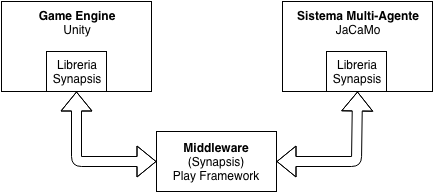
\includegraphics[width=0.8\linewidth]{figures/Architettura_alto_livello.png}
   \caption{Architettura ad alto livello}
   \label{architettura_alto_livello}
\end{figure}

L'architettura di sistema (Figura \ref{architettura_alto_livello}) introduce un nuovo componente, definito Synapsis e realizzato con il framework Play, separato e autonomo rispetto alle differenti tecnologie utilizzate su MAS e GE. L'obiettivo di questo middleware è mettere in collegamento le parti di entità presenti nei due sistemi e, quindi di trasportare le azioni da mente a corpo e le percezione da corpo a mente.

\medskip

Per collegare MAS e GE al middleware, sono state realizzate due librerie che contengono funzionalità di collegamento e comunicazione con Synapsis. Le librerie rispettano astrazioni e modelli computazionali di entrambi i sistemi (MAS e GE) ed utilizzano la terminologia precedentemente definita.

\medskip

Aggiungendo la struttura di una generica entità, definita nella sezione \ref{struttura_entita1}, all'architettura precedente è possibile notare come l'entità risulti suddivisa tra i due sistemi (MAS e GE) ed attraverso il collegamento al middleware, venga reso possibile lo scambio di informazioni (percezioni, azioni) pur avendo mente e corpo computazionalmente separati.

\begin{figure}[H]
   \centering
   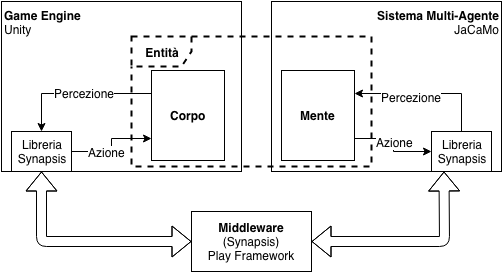
\includegraphics[width=\linewidth]{figures/Middleware_entity.png}
   \caption{Divisione di un'entità nel sistema}
\end{figure}

L'aggiunta del middleware come layer di collegamento, rispetto alla soluzione proposta nei lavori visti nella sezione \ref{MAS_dentro_GE}, favorisce il completo utilizzo, da parte degli sviluppatori, delle astrazioni e delle funzionalità presenti nelle Game Engine e nei MAS.

\medskip

\subsection{Confronto con la precedente soluzione}

Nella sezione \ref{MAS_GE_separati} è stata descritta l'architettura del precedente lavoro \cite{amslaurea12270} con lo stesso obiettivo del sistema realizzato in questo elaborato. Le due architetture presentano delle similitudini:
\begin{itemize}
    \item Utilizzo del concetto di "mente" e "corpo" per identificare le parti dell'entità nei rispettivi sistemi (MAS e GE);
    \item Utilizzo dell'artefatto come strumento di comunicazione dell'agente verso il proprio GameObject (corpo);
    \item Definizione dell'entità "mente" attraverso il collegamento tra agente ed artefatto specifico;
    \item Protocollo di comunicazione tra mente e corpo basato su messaggi strutturalmente simili (sezione \ref{protocollo_messaggi}).
\end{itemize}

Le principali differenze riguardano i seguenti aspetti:
\begin{itemize}
    \item Struttura del middleware: Nel precedente lavoro, il middleware è stato separato in due parti inglobate nella Game Engine e nel Sistema Multi-Agente. Nell'architettura proposta il middleware diventa un unico componente separato che mette in comunicazione i due sistemi;
    \item Struttura della comunicazione: Nella soluzione proposta ogni parte di entità (mente e corpo) possiede il proprio collegamento al middleware al posto di utilizzare un unico componente (smistatore), presente in entrambi i sistemi (MAS e GE), per interfacciarsi alla controparte. Difatto nella precedente soluzione esiste un solo canale di comunicazione invece di diversi canali nella architettura proposta (sezione \ref{struttura_sistema_finale}).
\end{itemize}